\documentclass[12pt,a4paper]{scrartcl} 
\usepackage[utf8]{inputenc}
\usepackage[english,russian]{babel}
\usepackage{indentfirst}
\usepackage{misccorr}
\usepackage{graphicx}
\usepackage{amsmath}
\begin{document}
	\begin{titlepage}
		\begin{center}
			\large
			МИНИСТЕРСТВО НАУКИ И ВЫСШЕГО ОБРАЗОВАНИЯ РОССИЙСКОЙ ФЕДЕРАЦИИ
			
			Федеральное государственное бюджетное образовательное учреждение высшего образования
			
			\textbf{АДЫГЕЙСКИЙ ГОСУДАРСТВЕННЫЙ УНИВЕРСИТЕТ}
			\vspace{0.25cm}
			
			Инженерно-физический факультет
			
			Кафедра автоматизированных систем обработки информации и управления
			\vfill

			\vfill
			
			\textsc{Отчет по практике}\\[5mm]
			
			{\LARGE \textit{Решение квадратного урвавнения и нахождение его корней}}
			\bigskip
			
			1 курс, группа 1ИВТ1
		\end{center}
		\vfill
		
		\newlength{\ML}
		\settowidth{\ML}{«\underline{\hspace{0.7cm}}» \underline{\hspace{2cm}}}
		\hfill\begin{minipage}{0.5\textwidth}
			Выполнил:\\
			\underline{\hspace{\ML}} Ю.\,С.~Бояршинов\\
			«\underline{\hspace{0.7cm}}» \underline{\hspace{2cm}} 2021 г.
		\end{minipage}%
		\bigskip
		
		\hfill\begin{minipage}{0.5\textwidth}
			Руководитель:\\
			\underline{\hspace{\ML}} С.\,В.~Теплоухов\\
			«\underline{\hspace{0.7cm}}» \underline{\hspace{2cm}} 2021 г.
		\end{minipage}%
		\vfill
	
		\begin{center}
			Майкоп, 2021 г.
		\end{center}
	\end{titlepage}



\begin{enumerate}
 \item Текстовая формулировка задачи
 \item Пример кода, решающего данную задачу
 \item График
 \item Скриншот программы
\end{enumerate}
\section{Ход работы}
\label{sec:exp}
\subsection{Текстовая формулировка задачи}
Написать приложение для вычисления корней квадратного уравнения (всех возможных вариантов и комплексности корней).
\subsection{Код приложения}
\label{sec:exp:code}
\begin{verbatim}
#include <iostream>
#include <cmath>
#include <math.h>
#include <stdio.h> 
using namespace std;
int main()
{
	setlocale(LC_ALL, "Russian");
	float a, b, c, x1 , x2, D;

	cout << "Введите 3 числа задачи AX^2+BX+C" << endl;
	cin >> a;
	cin >> b;
	cin >> c;
	D = pow(b,2)-(4*a*c);
	if (D>0)
	{
		D = sqrt(D);
		x1 = (-b-D)/(2*a);
		x2 = (-b+D)/(2*a);
		cout << "Два корня " << x1 << " & " << x2 << endl;
	}
	if (D==0)
	{
		x1 = (-b)/(2 * a);
		cout << "Единый корень " << x1 << " " << endl;
	}
	if (D<0)
		cout << "Корней нет " << endl;
	system("pause");
	return 0;
}
}
}
\end{verbatim}
\subsection{Пример формулы, график}
\label{sec:mathexample}

Решение квадратного уравнения \(ax^2+bx+c=0\):
\begin{equation}\label{eq:solv}
 x_{1,2}=\frac{-b\pm\sqrt{b^2-4ac}}{2a}
\end{equation}
\label{sec:picexample}
\begin{figure}[h]
	\centering
	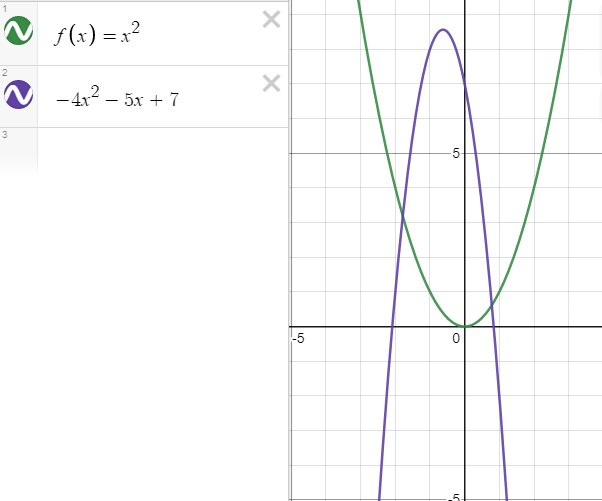
\includegraphics[width=0.4\textwidth]{Graphic.PNG}
	\caption{График Параболы и Примера задачи}\label{fig:par}
\end{figure}
\subsection{Скриншот программы, пример библиографических ссылок}
\label{sec:picexample}

\begin{figure}[h]
	\centering
	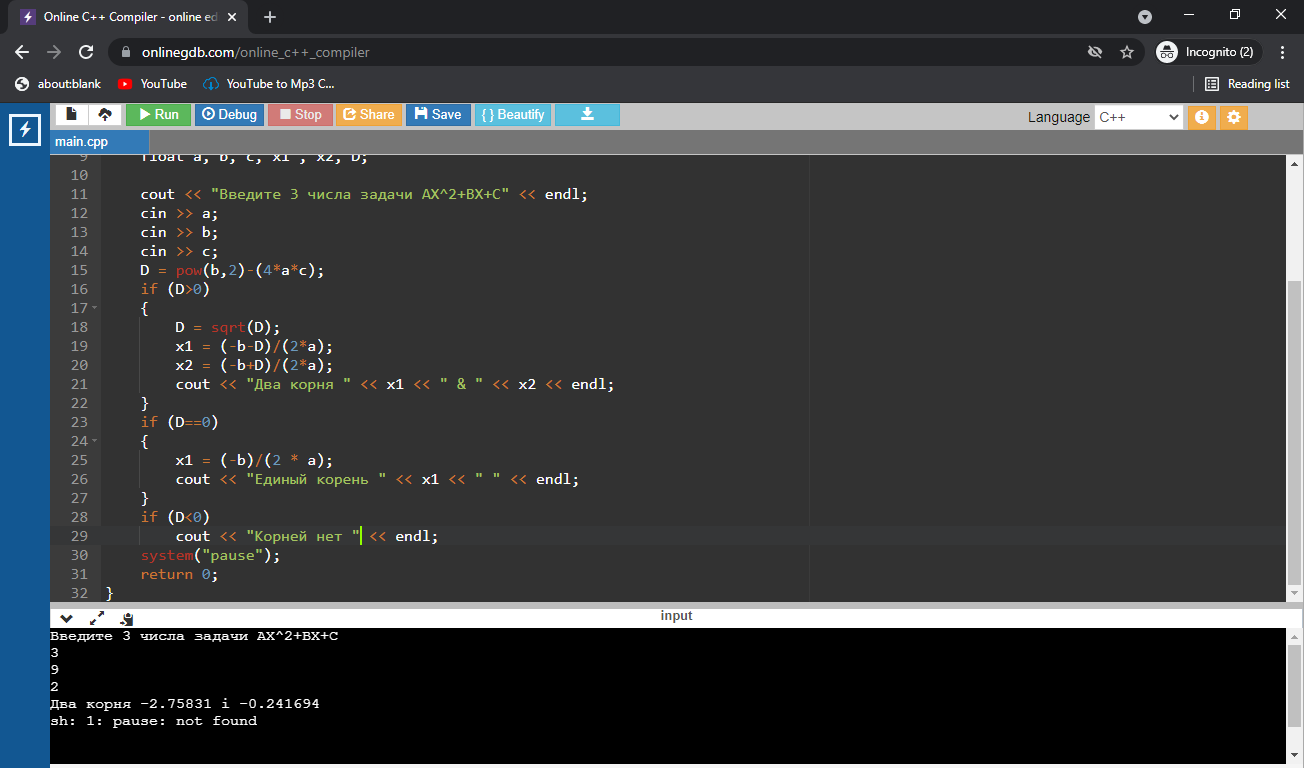
\includegraphics[width=0.4\textwidth]{ScreenOfProgramm.PNG}
\end{figure}

Для изучения «внутренностей» \TeX{} я 
изучил~\cite{Knuth-2003}, а для использования \LaTeX{}
почитал~\cite{Lvovsky-2003, Voroncov-2005}. Для написания программы на С++ я использовал \cite{Herbert-2013, Scott-2019}


\begin{thebibliography}{9}
\bibitem{Knuth-2003}Кнут Д.Э. Всё про \TeX. \newblock --- Москва: Изд. Вильямс, 2003 г. 550~с.
\bibitem{Lvovsky-2003}Львовский С.М. Набор и верстка в системе \LaTeX{}. \newblock --- 3-е издание, исправленное и дополненное, 2003 г.
\bibitem{Voroncov-2005}Воронцов К.В. \LaTeX{} в примерах. 2005 г.
\bibitem{Herbert-2013}Геберт Шильт --- "С++ для начинающих. Шаг за шагом". 2013г.
\bibitem{Scott-2019}Мейерс Скотт --- "Эффективный и современный С++: 42 рекомендации по использованию C++11 и C++14". 2019г.
\end{thebibliography}
\end{document}